% Intended LaTeX compiler: pdflatex
\documentclass[10pt,a4paper,UTF8]{article}
\usepackage{zclorg}
\author{张朝龙}
\date{}
\title{练习:张成空间与线性无关}
\hypersetup{
 pdfauthor={张朝龙},
 pdftitle={练习:张成空间与线性无关},
 pdfkeywords={},
 pdfsubject={},
 pdfcreator={Emacs 25.0.50.1 (Org mode 9.0.5)}, 
 pdflang={English}}
\begin{document}

\maketitle
\tableofcontents
\titlepic{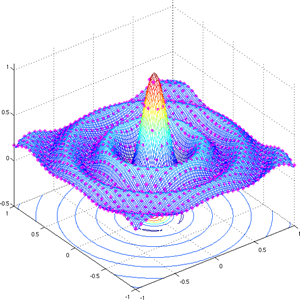
\includegraphics[scale=0.25]{../../img/sinc.PNG}}


\section*{2.a.1}
\label{sec:orge5915c5}


\begin{problem}
设\(v_{1},v_{2},v_{3},v_{4}\)张成\(V\),证明组\(v_{1}-v_{2},v_{2}-v_{3},v_{3}-v_{4},v_{4}\)也张成\(V\)
\end{problem}

\begin{answer}
设\(u\in V\),则存在\(c_{1},c_{2},c_{3},c_{4}\)使得


\begin{eqnarray*}
u &=& c_{1}v_{1} + (c_{2} - c_{1})v_{2} + (c_{3}-c_{2})v_{3} + (c_{4}-c_{3})v_{4} \\
 &=& c_{1}(v_{1}-v_{2}) + c_{2}(v_{2} - v_{3}) + c_{3}(v_{3} - v_{4}) + c_{4}v_{4}
\end{eqnarray*}

我们有,能用\(v_{1},v_{2},v_{3},v_{4}\)表示的元素,同样可以用\(v_{1}-v_{2},v_{2}-v_{3},v_{3}-v_{4},v_{4}\)来表示。命题得证。
\end{answer}
\section*{2.a.3}
\label{sec:orgb95b2d1}


\begin{problem}
求数\(t\)使得\((3,1,4),(2,-3,5),(5,9,t)\)在\(\mathbf{R}^{3}\)中不是线性无关的。
\end{problem}

\begin{answer}
假设有\(x,y,z\)使得:
\begin{eqnarray}
\label{eq:1}
3x+2y&=&5 \\
x-3y&=&9 \\
4x+5y&=&t \\
\end{eqnarray}
由前两个十字我们得到 \(x=3, y =-2, t= 2\)
如此,我们有 \(3(3,1,4) + (-2)(2,-3,5) = (5,9,2)\),因此\(t=2\)是我们要找的那个数。
\end{answer}
\section*{2.a.5}
\label{sec:orgef03625}


\begin{problem}
证明:若将\(\mathbf{C}\)视为\(\mathbf{R}\)上的向量空间,则\(1+i,1-i\)是线性无关的。
\end{problem}

\begin{answer}
假设存在\(x,y\in \mathbf{R}\)使得:
\begin{equation}
\label{eq:3}
x(1+i) + y(1-i) = 0
\end{equation}
则有:
\begin{eqnarray*}
x+y&=&0 \\
x-y&=&0
\end{eqnarray*}
所以\(x=y=0\),即 \(1+i,1-i\)是线性无关的。
\end{answer}

\begin{problem}
证明:若将\(\mathbf{C}\)视为\(\mathbf{C}\)上的向量空间,则\(1+i,1-i\)是线性相关的。
\end{problem}

\begin{answer}
假设存在\(x,y\in \mathbf{F}\)使得:

\begin{equation}
\label{eq:4}
x(1+i) + y(1-i) = 0
\end{equation}
我们有x=1-i,y=-(1+i),使得\((1-i)(1+i) - (1+i)(1-i) = 0\)
\end{answer}
\section*{2.a.6}
\label{sec:org1456dc7}


\begin{problem}
设\(v_{1},v_{2},v_{3},v_{4}\)是线性无关的,证明\(v_{1}-v_{2},v_{2}-v_{3},v_{3}-v_{4},v_{4}\)也是线性无关的。
\end{problem}

\begin{answer}
假设存在\(a_{1},a_{2},a_{3},a_{4}\)使得
\begin{equation}
\label{eq:5}
a_{1}(v_{1}-v_{2}) + a_{2}(v_{2} - v_{3}) + a_{3}(v_{3}-v_{4}) + a_{4}v_{4} =0
\end{equation}
对上式变形有:
\begin{equation}
\label{eq:6}
a_{1}v_{1} + (a_{2}-a_{1})v_{2} + (a_{3}-a_{2})v_{3} + (a_{4}-a_{3})v_{4} = 0
\end{equation}
又因为\(v_{1},v_{2},v_{3},v_{4}\)是线性无关的,所以有:
\begin{eqnarray*}
a_{1}&=&0 \\
a_{2} - a_{1} &=&0 \\
a_{3} -a_{2} &=&0 \\
a_{4} - a_{3} &=& 0
\end{eqnarray*}

显然有\(a_{1}=a_{2}=a_{3}=a_{4}=9\), 即原命题得证。
\end{answer}
\section*{2.a.7}
\label{sec:orgf459151}



\begin{problem}
证明或者给出反例:若\(v_{1},v_{2},\ldots ,v_{m}\)在\(V\)中线性无关,则\(5v_{1}-4v_{2},v_{2},v_{3},\ldots ,v_{m}\)是线性无关的。
\end{problem}

\begin{answer}
这是个真命题,证明过程和2.a.6的过程一样。就不详述了。
\end{answer}
\section*{2.a.8}
\label{sec:orgc27fa71}


\begin{problem}
证明或者给出反例:设\(v_{1},\ldots ,v_{m}\)在\(V\)中线性无关,并设\(\lambda \in \mathbf{F}\)且\(\lambda \neq 0\),则\(\lambda v_{1},\lambda v_{2},\ldots ,\lambda v_{m}\)是线性无关的。
\end{problem}

\begin{answer}
证明过程同2.a.6
\end{answer}

\section*{2.a.9}
\label{sec:org2c5559f}


\begin{problem}
证明或者给出反例:若\(v_{1},\ldots ,v_{m}\)和\(w_{1},\ldots ,w_{m}\)是\(V\)中的线性无关组,则\(v_{1}+w_{1},\ldots ,v_{m}+w_{m}\)是线性无关的。
\end{problem}

\begin{answer}
反例:有当\(w_{i} = -v_{i},i=1,\ldots ,m\)时,\(v_{i} + w_{i} = 0, i = 1,\ldots ,m\),此时\(m\)个\(0\)向量构成的向量组是线性相关的。
\end{answer}

\section*{2.a.10}
\label{sec:org887aff1}


\begin{problem}
设\(v_{1},\ldots ,v_{m}\)在\(V\)中线性无关,并设\(w\in V\),证明若\(v_{1}+w,\ldots ,v_{m}+w)线性相关,则有 \(w\in span(v_{1},\ldots ,v_{m}\)
\end{problem}

\begin{answer}
显然若\(v_{1}+w,\ldots ,v_{m}+w\)线性相关,则存在不全为零的\(a_{1},a_{2},\ldots ,a_{m}\)使得:
\begin{equation}
\label{eq:8}
a_{1}(v_{1} + w) + \ldots + a_{m}(v_{m} + w) = 0
\end{equation}

则有
\begin{equation}
\label{eq:9}
\sum_{i=1}^{m}a_{i}v_{i} = -\sum_{i=1}^{m}a_{i}w
\end{equation}

若\(\sum_{i}^{m}a_{i} = 0\),则有上式右边为零,根据\(v_{1},\ldots ,v_{m}\)在\(V\)中线性无关,我们有\(a_{i}=0,i=1,\ldots ,m\),与假设矛盾(我们假设\(a_{i},i=1,\ldots ,m\)不全为零)。因此\(\sum_{i}^{m}a_{i} \neq 0\)

因此:
\begin{equation}
\label{eq:10}
w = -\frac{\sum_{i=1}^{m}a_{i}v_{i}}{\sum_{i=1}^{m}a_{i}} 
\end{equation}

即\(w\in span(v_{1},\ldots ,v_{m})\)
\end{answer}
\section*{2.a.11}
\label{sec:org7bffa9c}


\begin{problem}
设\(v_{1},\ldots ,v_{m}\)在\(V\)中线性无关,并设\(w\in V\),证明:\(v_{1},\ldots ,v_{m},w\)线性无关,当且仅当\(w\notin span(v_{1},\ldots ,v_{m})\)
\end{problem}

\begin{answer}
证明,我们首先从\(v_{1},\ldots ,v_{m},w\)线性无关,推出\(w\notin span(v_{1},\ldots ,v_{m})\)。使用反证法。假设 \(w\in span(v_{1},\ldots ,v_{m})\),则存在\(a_{1},\ldots ,a_{m}\)使得:
\begin{equation}
\label{eq:11}
w = a_{1}v_{1} + \ldots + a_{m}v_{m}
\end{equation}
即:\(a_{1}v_{1} + \ldots + a_{m}v_{m} - w = 0\),因为\(w\)的系数为\(-1\),与\(v_{1},\ldots ,v_{m},w\)线性无关矛盾。

接着我们从\(w\notin span(v_{1},\ldots ,v_{m})\),推出\(v_{1},\ldots ,v_{m},w\)线性无关。同样使用反证法:假设\(v_{1},\ldots ,v_{m},w\)线性相关,则有不全为零的数\(a_{1},\ldots ,a_{m},b\),使得:
\begin{equation}
\label{eq:12}
bw + a_{1}v_{1} + \ldots + a_{m}v_{m} = 0
\end{equation}

此时\(b\)一定不等于零,因为若\(b=0\),根据\(v_{1},\ldots ,v_{m}\)在\(V\)中线性无关,则有\(a_{i}=0,i=1,\ldots ,m\),此时\(v_{1},\ldots ,v_{m},w\)线性无关,与假设矛盾。

由于\(b\)不等于零,则有:
\begin{equation}
\label{eq:13}
w = -\frac{\sum_{i}^{m}a_{i}v_{i}}{b}
\end{equation}
显然有\(w\in span(v_{1},\ldots ,v_{m})\),与假设矛盾。
\end{answer}

\section*{2.a.12}
\label{sec:org69d2e41}


\begin{problem}
为什么在\(\mathcal{P}_{4}(\mathbf{F})\)中不存在由6个多项式构成的线性无关组。
\end{problem}

\begin{answer}
因为\(1,x,x^{2},x^{3},x^{4}\)张成了\(\mathcal{P}_{4}(\mathbf{F})\),而一个空间总线性无关组的长度不可能大于张成组的长度。
\end{answer}

\section*{2.a.13}
\label{sec:org71c4e73}


\begin{problem}
为什么4个多项式构成的组不能张成\(\mathcal{P}_{4}(\mathbf{F})\)?
\end{problem}

\begin{answer}
因为\(1,x,x^{2},x^{3},x^{4},x^{5}\)这个线性无关组张成了\(\mathcal{P}_{4}(\mathbf{F})\),所以4个多项式构成的组不能张成\(\mathcal{P}_{4}(\mathbf{F})\)。
\end{answer}
\section*{2.a.14}
\label{sec:orgf8e0bc5}


\begin{problem}
证明:\(V\)是无限维的当且仅当\(V\)中存在一个向量序列\(v_{1},v_{2},\ldots\)使得当\(m\)是任意正整数时,都有\(v_{1},\ldots ,v_{m}\)都是线性无关的。
\end{problem}

\begin{answer}
假设\(V\)是无限维,说明\(V\)不能有该空间的任何向量组张成。因此当存在\(m\)使得\(V=span(v_{1},\ldots ,v_{m})\)时,与定义矛盾。

假设一个向量序列\(v_{1},v_{2},\ldots\)使得当\(m\)是任意正整数时,都有\(v_{1},\ldots ,v_{m}\)都是线性无关的,则说明任意有限个元素的向量组都无法张成\(V\),说明\(V\)是无限维的。
\end{answer}

\section*{2.a.15}
\label{sec:org34db71e}


\begin{problem}
证明\(\mathbf{F}^{\infty}\)是无限维的。
\end{problem}

\begin{answer}
假设\(0,\ldots ,0,1,0,\ldots\)是除了第\(i\)个元素以外都为领的向量。显然\(e_{1},\ldots ,e_{m}\)是线性无关的。根据2.a.14我们有\(\mathbf{F}^{\infty}\)是无穷维的。
\end{answer}

\section*{2.a.16}
\label{sec:org81605fa}


\begin{problem}
证明区间\([0,1]\)上的所有实值连续函数构成的向量空间是无穷维的。
\end{problem}

\begin{answer}
这个题目我一直解不出来,一定有什么tricky的东西。

定义:
\begin{equation}
\label{eq:14}
f_{n} =
\begin{cases}
x-1/n & x \geq 1/n; \\
0, & x\in [0,1/n]
\end{cases}
\end{equation}
那么\(f_{n}\)在\([0,1]\)内是连续的。接下来,我们证明\(f_{n+1}\notin span \{f_{1},\ldots ,f_{n}\}\),那么就有明区间\([0,1]\)上的所有实值连续函数构成的向量空间是无穷维的。

如果\(f_{n+1}\notin span \{f_{1},\ldots ,f_{n}\}\),那么有:
\begin{equation}
\label{eq:15}
f_{n+1}(x) = a_{1}f_{x} + \ldots + a_{n}f_{n}(x)
\end{equation}
注意,我们有\(f_{1}(1/n) = \ldots = f_{n}(1/n)=0\),但是\(f_{n+1} = 1/(n(n+1)) \neq 0\)。矛盾。命题得证
\end{answer}

\section*{2.a.17}
\label{sec:org502968f}


\begin{problem}
设\(p_{0},\ldots ,p_{m}\) 是\(\mathcal{P}_{m}(\mathbf{F})\)中的多项式使得对每个\(j\)都有\(p_{j}(2) = 0\),证明\(p_{0},p_{1},\ldots ,p_{m}\)在\(\mathcal{P}_{m}(\mathbf{F})\)中不是线性无关的。
\end{problem}

\begin{answer}
假设\(p_{0},p_{1},\ldots ,p_{m}\)是线性独立的。我们知道对于一个维度是\(m\)的线性子空间,这个空间中的线性无关组向量的个数不可能大于其张成组向量的个数。我们知道\(1,z,\ldots ,z^{m}\)张成了\(\mathcal{P}_{m}(z)\),又因为假设\(p_{0},p_{1},\ldots ,p_{m}\)是线性独立的,说明其也是\(\mathcal{P}_{m}(z)\)的张成向量组。所以存在:
\begin{equation}
\label{eq:16}
z = a_{0}p_{0}(z) + \ldots a_{m}p_{m}(z)
\end{equation}

又因为每个\(j\)都有\(p_{j}(2) = 0\),我们有\(z=2\),矛盾。

所以\(p_{0},p_{1},\ldots ,p_{m}\)在\(\mathcal{P}_{m}(\mathbf{F})\)中不是线性无关的。
\end{answer}
\end{document}
